\section{Preliminaries}\label{sc:background}
This section gives some background on Maude and co-simulation.

\subsection{Maude /Rewriting Logic}
\simon{Peter, I guess you have some text for this section.}

\subsection{Co-simulation}
Complex CPS are typically composed of multiple communicating sub-systems/simulation units (SUs) examples include autonomous vehicles. 
Such systems can be explored using co-simulation.
Co-simulation is a technique enabling simulation of a complex CPS consisting of multiple black-box SUs. 
An SU represents a dynamic system and can compute the behavior of that system using a dedicated solver. 
A dynamic system represents a function from time and space into some often multi-dimensional and continuous state space. 
Examples include water flow and pendulums. \simon{More advanced examples}
The SU interacts with an \emph{external environment} through inputs and outputs dynamic~\cite{Gomes2019a,Kubler2000}.

SUs are coupled through their inputs and outputs.
A coupling indicates that the state of one SU is reliant on the state of another SU.
\simon{example}
The corresponding coupling restriction states that the value of a coupled input and output must be the same at all times.
However, in practice, the coupling restrictions can only be satisfied at specific points in time called \emph{communication points}. 
Therefore, each SU makes assumptions about the evolution of its' input values between the communication points.
The assumptions can introduce errors in the co-simulation~\cite{Arnold2014}.

\emph{The orchestrator} computes the behavioral trace of all SUs and tries to satisfy their coupling restrictions by exchanging values between the coupled ports. 
The orchestrator aims to find the communication points minimizing the co-simulation error while ensuring that the SUs move in lockstep. 
The optimal communication points depend on the implementation of the SUs~\cite{Gomes2019,Oakes2021,Gomes2018f,Schweizer2015c,Gomes2018a}.

The following \cref{def:fmu} of an SU is based on \cite{Broman2013,Gomes2019c,thrane2021}.

\begin{definition}[Simulation Unit]\label{def:fmu}
  An SU with identifier $c$ is given by the tuple
  $$ SU_c \triangleq \tuple{\stateset{c}, \inputs{c}, \outputs{c}, \fset{c}, \fget{c}, \fdoStep{c}, \values},$$
  where:
  \begin{compactitem}
    \item $\stateset{c}$ is a set, denoting the state space of the SU.
    \item $\inputs{c}$ and $\outputs{c}$ are sets, of input and output port, respectively.
    The union $\variables{c} = \inputs{c} \cup \outputs{c}$ of the inputs and outputs is called the ports of the SU.
    \item $\values$ is a set, intuitively denoting the values that a variable can hold.
    Let $\valuesExchanged = \timebase \times \values$ be the set of timestamp values exchanged between input and output ports.
    \item 
    The functions
    $\fset{c} : \stateset{c} \times \inputs{c} \times \valuesExchanged \to \stateset{c}$ and $\fget{c}: \stateset{c} \times \outputs{c} \to \valuesExchanged$ respectively sets an input and gets an output. 
    \item $\fdoStep{c}: \stateset{c} \times \stepbase \to \stateset{c} \times \stepbase $ is a function; it instructs the SU to compute its state after a given duration. 
    If an SU is in state $\stateafter{c}{t}$ at time $t$ then, $(\stateafter{c}{t+h}, h) = \fdoStep{c}(\stateafter{c}{t}, H)$ denotes the state $\stateafter{c}{t+h}$ of the corresponding SU at time $t+h$, where $h \leq H$. 
  \end{compactitem}
\end{definition}

The state of SU $A$ at time $t$ is denoted $\stateafter{A}{t}$.
The function $\fdoStep{c}$ returns a state and a step size, since some SUs implement error estimation and may conclude that taking a step size $H$ will result in an intolerable error.
Therefore, instead the SU takes a smaller step $h$ than planned.

A collection of coupled SUs forms a scenario:
we provide a formal description of a scenario in \cref{def:cosim_scenario}.

\begin{definition}[Scenario]\label{def:cosim_scenario}
  A scenario $\mathcal{S}$ is a tuple $\mathcal{S} \triangleq \tuple{\fmus, \{SU\}_{c \in \fmus}, \coupling, \mayReject, \allreactivity, \allfeedthroughs}$ where 
  \begin{compactitem}
    \item $\fmus$ is a finite set, of SU identifiers. 
    \item $\{SU\}_{c \in \fmus}$ is a set of SUs.
    \item The function 
    $\coupling : \allinputs \to \alloutputs$ where $\allinputs = \bigcup_{c \in \fmus} \inputs{c}$ and $\alloutputs = \bigcup_{c \in \fmus} \outputs{c}$, intuitively 
    $\coupling(u)=y$ means that the output $y$ is connected to input $u$.   
    \item $\mayReject \subseteq \fmus$ denotes the SUs that implement error estimation. 
    \item
    $\allreactivity : \allinputs \to \mathbb{B}$ is a total function, intuitively it provides information about the SUs' input approximation functions.
    $\allreactivity(\inputvar{c}) = \true$ means that the function $\fdoStep{c}$ assumes that the timestamp $t_{SU}$ of the state of $SU_c$ ($\stateafter{c}{t_{SU}}$) is smaller than the timestamp $t_v$ of the value $\tuple{t_v,v}$ set on the input $\inputvar{c}$.
    \item $\allfeedthroughs$ is a family of functions $\{\feedthrough{c} : \outputs{c} \to \mathcal{P}(\inputs{c})\}_{c \in \fmus}$.
    $\inputvar{c} \in \feedthrough{c}(\outputvar{c})$ means that the input $\inputvar{c}$ \emph{feeds through} to the output $\outputvar{c}$, such that there exists $v_1, v_2 \in \valuesExchanged$ and $\state{c} \in \stateset{c}$, such that
    $\fget{c} (\fset{c}(\state{c}, \inputvar{c}, v_1), \outputvar{c}) \neq \fget{c} (\fset{c}(\state{c}, \inputvar{c}, v_2), \outputvar{c}).$
  \end{compactitem}
\end{definition}

We have based \cref{def:cosim_scenario} on the FMI 2.0 standard~\cite{FMI2014}. 
However, feed-through and instrumentation are extensions of the standard, introduced to cover a broad class of co-simulation scenarios.
We use the syntax in \cref{fig:simpleexample} to graphically present co-simulation scenarios.

\begin{figure}[htb]
  \centering
  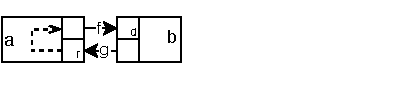
\includegraphics[width=0.7\textwidth]{images/simple_example.pdf}
  \caption{A co-simulation scenario, where the dashed arrows denote feed-through, $a$ and $b$ are SU identifiers, the small squares denoted $r$ and $d$ are .
  The solid arrows $f$ and $g$ are the coupling.}
  \label{fig:simpleexample}  
\end{figure}

\subsubsection{Instrumentation}
We call an input port $\inputvar{c}$ \emph{delayed} if $\neg \allreactivity(\inputvar{c})$ and \emph{reactive} if $\allreactivity(\inputvar{c})$. 

The function $\allreactivity$ is the instrumentation of the scenario.
The instrumentation describes the input approximation functions of the different SUs.
%An example of the instrumentation function
Changing the instrumentation of a scenario changes the algorithm used to simulate the scenario.
We assume that the instrumentation of a scenario is constant through the simulation, which is the case for most commercially used SUs~\cite{Gomes2018a}.

\subsection{Co-simulation Algorithms}\label{sc:cosimalgo}
An \emph{orchestrator} simulates a scenario by executing the \emph{co-simulation algorithm}.

A co-simulation algorithm consists of an initialization procedure, a co-simulation step, and some additional FMI functions changing the mode of an SU~\cite{FMI2014}.
This work focuses on on the co-simulation step, which we refer to as ``the algorithm'' throughout the paper. 
The other aspects of a co-simulation algorithm can be derived from our method.  

The algorithm changes the co-simulation state. 
We use an abstract co-simulation state, which is defined as the combination of the state of the SUs.

The following \cref{def:runtime_state} defines the abstract state of an SU.

\begin{definition}[Abstract State]\label{def:runtime_state}
  The observable abstract state of SU $SU_c$ is an element of the set $\runstate{c} = \timebase \times \runstate{\inputs{c}} \times \runstate{\outputs{c}} \times \runstate{V_c}$, where:
  \begin{compactitem}
    \item $\runstate{\inputs{c}} : \inputs{c} \to \timebase$ is a total function mapping each input port to a timestamp.  
    \item $\runstate{\outputs{c}} : \outputs{c} \to \timebase$ is a total function mapping each output port to a timestamp.  
    \item $\runstate{V_c} : \variables{c} \to \values$ is a total function mapping each port to a value.  
  \end{compactitem}
  Intuitively the first components of the abstract state denotes the time of the SU.
\end{definition}

We use the abstract state $\runstate{c}$ of an SU $c$ instead of the internal state $\stateset{c}$ since the orchestrator cannot observe the latter.

\begin{definition}[Abstract Co-simulation State]\label{def:cosimstate}
  Given a co-simulation scenario $S$ with $C$ as the identifiers of the SUs the abstract co-simulation state is an element in the set $\runstate{\fmus} = \prod_{c \in \fmus} \runstate{c}$. 
\end{definition}

A co-simulation step $P$ is a sequence of the applications of the functions $\fset{c},\fget{c}$, and $\fdoStep{c}$.
It simulates the scenario by advancing all SUs from an initial state at time $t$ to a final state at time $t+H, \textrm{ where } H > 0$.
The co-simulation must ensure that the coupling restrictions are satisfied at both the initial and final state.

\Cref{fig:algorithms} shows three different co-simulation steps of the scenario in \cref{fig:simpleexample}.
All these three algorithms are allowed by the FMI standard 2.1~\cite{FMI2014}. 

\begin{figure}[htb]
  \centering
  \begin{minipage}[t]{.325\textwidth}
    \begin{algorithm}[H]
      \caption{}
      \label{alg:algorithm_1}
      \begin{algorithmic}[1]
        \scriptsize
        \State $(\stateafter{A}{H},H) \gets \fdoStep{A}(\stateafter{A}{0}, H)$
        \State $(\stateafter{B}{H},H) \gets \fdoStep{B}(\stateafter{B}{0}, H)$
        \State $f_{v} \gets \fget{A}(\stateafter{A}{H}, \outputvar{f})$
        \State $g_{v} \gets \fget{B}(\stateafter{B}{H}, \outputvar{g})$
        \State $\stateafter{B}{H} \gets \fset{B}(\stateafter{B}{s}, \inputvar{f}, f_{v})$
        \State $\stateafter{A}{H} \gets \fset{A}(\stateafter{A}{H},\inputvar{g},g_{v})$
      \end{algorithmic}
    \end{algorithm}
  \end{minipage}
  \begin{minipage}[t]{0.325\textwidth}
    \begin{algorithm}[H]
      \caption{}
      \label{alg:algorithm_2}
      \begin{algorithmic}[1]
        \scriptsize
        \State $(\stateafter{B}{H},H) \gets \fdoStep{B}(\stateafter{B}{0}, H)$
        \State $(\stateafter{A}{H},H) \gets \fdoStep{A}(\stateafter{A}{0}, H)$
        \State $g_v \gets \fget{B}(\stateafter{B}{H}, \outputvar{g})$
        \State $\stateafter{A}{H} \gets \fset{A}(\stateafter{A}{H}, \inputvar{g}, g_v)$
        \State $f_v \gets \fget{A}(\stateafter{A}{H}, \outputvar{f})$
        \State $\stateafter{B}{H} \gets \fset{B}(\stateafter{B}{H}, \inputvar{f}, f_v)$
      \end{algorithmic}
    \end{algorithm}
  \end{minipage}
  \begin{minipage}[t]{0.325\textwidth}
    \begin{algorithm}[H]
      \caption{}
      \label{alg:algorithm_3}
      \begin{algorithmic}[1]
        \scriptsize
        \State $(\stateafter{B}{H},H) \gets \fdoStep{B}(\stateafter{B}{0}, H)$
        \State $g_v \gets \fget{B}(\stateafter{B}{H}, \outputvar{g})$
        \State $\stateafter{A}{0} \gets \fset{A}(\stateafter{A}{0}, \inputvar{g}, g_v)$
        \State $f_v \gets \fget{A}(\stateafter{A}{0}, \outputvar{f})$
        \State $\stateafter{B}{H} \gets \fset{B}(\stateafter{B}{H}, \inputvar{f}, f_v)$
        \State $(\stateafter{A}{H},H) \gets \fdoStep{A}(\stateafter{A}{0}, H)$
      \end{algorithmic}
    \end{algorithm}
    \vspace{4pt}
  \end{minipage}
  \vspace{-2em}
  \caption{Three co-simulation algorithms of the scenario in \cref{fig:simpleexample} conforming to the FMI Standard (version 2.0).}
  \label{fig:algorithms}
\end{figure}

Although the three algorithms in \cref{fig:algorithms} consist of the same actions, they are not equivalent, and simulating with one algorithm instead of one of the others could drastically change the co-simulation result as shown in \cite{Gomes2019c,hansen_verification_2021}. 

The co-simulation step $P$ should satisfy \cref{def:comsim_step}.

\begin{definition}[Co-simulation Step]\label{def:comsim_step}
  A co-simulation step $P$ must start in an initial state satisfying.
  \begin{align}
    &\fpreCoSimStep(\tuple{t,\runstate{\allinputs}, \runstate{\alloutputs},\runstate{V}}, t) \triangleq 
    \forall \inputvar{c} \in \allinputs
    \exists \outputvar{d} \in \alloutputs
    \cdot \coupling(\inputvar{c}) = \outputvar{d}  \nonumber \\
    &\qquad \qquad \qquad \qquad \qquad \implies
    \runstate{V}(\inputvar{c}) = \runstate{V}(\outputvar{d})
  \end{align}
  The co-simulation step $P$ must satisfy the following property: 
  \begin{align}
    &[\fpreCoSimStep(\runstate{}, t), 
    \fpreCoSimStep(\after{\runstate{}}, t+H)] 
    \langle \after{\runstate{}} \gets P\rangle
  \end{align}
\end{definition}

$\runstate{} = \tuple{t, \runstate{\allinputs}, \runstate{\alloutputs}, \runstate{V}}$ means that all SUs are at time $t$ and $\runstate{\allinputs} = \prod_{c \in \fmus}\runstate{\inputs{c}}$ and $\runstate{\alloutputs} = \prod_{c \in \fmus}\runstate{\outputs{c}}$.
\Cref{def:comsim_step} shows that the precondition and postcondition of the co-simulation step are the same ($\fpreCoSimStep$).
It says that all SUs are synchronized and that all the coupling restrictions are satisfied.

All the three Algorithms in \cref{fig:algorithms} satisfy the property above even though they can result in different simulation results.
To differentiate between them, we need to look into the semantics of the different actions described in \cref{def:fmu}, which we describe in \cref{def:getout,def:setin,def:step}.

We base our semantics on \cite{Gomes2019a,hansen_verification_2021} to which we refer for more information.
\simon{Make reference to Journal}

\begin{definition}[Get Action]\label{def:getout}  
  For an SU $c$ at timestamp $t$ with the abstract state $\runstate{c} = \tuple{t,\runstate{\inputs{c}}, \runstate{\outputs{c}}, \runstate{V_c}}$ the effect of obtaining a value from an output $\outputvar{c}$ using the action $\fget{c}(\stateafter{c}{t},\outputvar{c})$ is described using the specification statement:
  \begin{align*}
    &\fpreget{c}(\outputvar{c}, \tuple{t,\runstate{\inputs{c}}, \runstate{\outputs{c}}, \runstate{V_c}}) \triangleq
    \runstate{\outputs{c}}(\outputvar{c}) < t \land \nonumber \\
    & \qquad \qquad \qquad \qquad \qquad 
    \forall \inputvar{c} \in \inputs{c} \cdot (\inputvar{c}, \outputvar{c}) \in \feedthrough{c} 
    \implies \runstate{\inputs{c}}(\inputvar{c}) = t 
  \end{align*}
  The precondition intuitively states that a value from the output must not have been obtained since the last step of the SU.
  Furthermore, it requires that all the inputs that feed through to the input have been updated.
  The postcondition ensures the advancement of time of the input $\outputvar{c}$.
  \begin{align*}
    &\fpostget{c}(\outputvar{c}, \tuple{t,\runstate{\inputs{c}}, \runstate{\outputs{c}}, \runstate{V_c}}, 
    \tuple{t,\runstate{\inputs{c}}, \after{\runstate{\outputs{c}}}, \runstate{V_c}}, v) \triangleq 
    \after{\runstate{\outputs{c}}}(\outputvar{c}) = t \nonumber \\
    & \qquad \qquad \qquad \qquad \qquad 
    \land 
    \forall \outputvar{m} \in (\outputs{c} \setminus \outputvar{c}) \cdot 
    \after{\runstate{\outputs{c}}}(\outputvar{m}) =
    \runstate{\outputs{c}}(\outputvar{m})
  \end{align*}
  The $\fget{c}$ action satisfies the following property.
  \begin{align*}
    &[\fpreget{c}(\outputvar{c}, \runstate{c}), 
    \fpostget{c}(\outputvar{c}, \runstate{c}, \after{\runstate{c}}, v)] 
    \langle (v, \after{\runstate{c}}) \gets \fget{c}(\stateafter{c}{t},\outputvar{c}) \rangle \nonumber
  \end{align*}
\end{definition}

\begin{definition}[Set Action]\label{def:setin}
  To set a value $\tuple{t_{V}, X}$ on the input $\inputvar{c}$ of SU $c$ using $\fset{c}(\stateafter{c}{t}, \inputvar{c}, \tuple{t_{V}, X})$ its abstract state must satisfy:
    \begin{align*}
      &\fpreset{c}(\inputvar{c}, \tuple{t_{V},X}, \tuple{t,\runstate{\inputs{c}}, \runstate{\outputs{c}}, \runstate{V_c}}) \triangleq 
      let\; t_s = \runstate{\inputs{c}}(\inputvar{c}) \; in \; t_s < t_{V} \nonumber \\
      & \qquad \qquad \qquad \qquad \qquad
      \land 
      ((\allreactivity(\inputvar{c}) \land t_s = t) 
      \lor (\neg\allreactivity(\inputvar{c}) \land t_s < t))
    \end{align*}
    The precondition intuitively states that the input must not have been set since the last step of the SU.
    Furthermore, it requires that the value set on the input should respect the instrumentation of the input.
    The postcondition ensures the value of the input $\inputvar{c}$  is updated. In addition, the timestamp of the input must also be updated.
    \begin{align*}
      &\fpostset{c}(\inputvar{c}, \tuple{t_{V},X}, \tuple{t,\runstate{\inputs{c}}, \runstate{\outputs{c}}, \runstate{V_c}}, 
      \tuple{t, \after{\runstate{\inputs{c}}} \runstate{\outputs{c}}, \after{\runstate{V_c}}}) \triangleq 
      t_{V} = \after{\runstate{\inputs{c}}}(\inputvar{c})
      \nonumber\\
      &\qquad \qquad \qquad \qquad \qquad \land
      \forall \inputvar{m} \in (\inputs{c} \setminus \inputvar{c}) \cdot 
      \after{\runstate{\inputs{c}}}(\inputvar{m}) =
      \runstate{\inputs{c}}(\inputvar{m}) 
      \nonumber \\
      &\qquad \qquad \qquad \qquad \qquad \land
      \after{\runstate{V_c}}(\inputvar{c}) = X 
    \end{align*}
    The $\fset{c}$ action satisfies the following property.
    \begin{align*}
      &[\fpreset{c}(\inputvar{c}, \runstate{c}), 
      \fpostset{c}(\inputvar{c}, \inputV, \runstate{c}, \after{\runstate{c}})] 
      \langle \after{\runstate{c}} \gets \fset{c}(\stateafter{c}{t},\inputvar{c}, \inputV) \rangle \nonumber
    \end{align*}
  \end{definition}

  \begin{definition}[Step Computation]\label{def:step}
    To step an SU $c$ using $\fdoStep{c}(\stateafter{c}{t}, H)$ its abstract state must satisfy:
    \begin{align*}
      &\fpredoStep{c}(H, \tuple{t,\runstate{\inputs{c}}, \runstate{\outputs{c}, \runstate{V_c}}}) \triangleq 
      \forall \inputvar{c} \in \inputs{c}
      \cdot 
      ((\allreactivity(\inputvar{c}) \land t_{SU} + H = \runstate{\inputs{c}}(\inputvar{c}))
      \nonumber \\
      &\qquad \qquad \qquad \qquad \qquad \qquad \qquad \qquad \qquad 
      \lor 
      (\neg \allreactivity(\inputvar{c}) \land t_{SU} = \runstate{\inputs{c}}(\inputvar{c})))
    \end{align*}
    The precondition states that all the SU's inputs must be updated according to their instrumentation.  
    The postcondition below ensures that the time of the SU advances by $H$.
    \begin{align*}
      &\fpostdoStep{c}(H, \tuple{t,\runstate{\inputs{c}}, \runstate{\outputs{c}}, \runstate{V_c}}, \tuple{t',\runstate{\inputs{c}}, \runstate{\outputs{c}}, \after{\runstate{V_c}}}) \triangleq t + H = t'
    \end{align*}
    The $\fdoStep{c}$ action satisfies the following property.
    \begin{align*}
      &[\fpredoStep{c}(H, \runstate{c}), 
      \fpostdoStep{c}(H, \runstate{c}, \after{\runstate{c}})] 
      \langle (\after{\runstate{c}}, H) \gets \fdoStep{c}(\stateafter{c}{t},H) \rangle \nonumber
    \end{align*}
  \end{definition}

The following section introduces a special class of co-simulation scenarios.

\subsection{Complex Scenarios}
Complex scenarios are subject to algebraic loops or step rejections.
A complex scenario is simulated using an iterative orchestration algorithm.
\simon{Add scenario /figure}

The algorithm is iterative because the orchestrator needs to adapt to the behavior of the SUs to satisfy the constraints associated with each SU, account for possible step rejections, and solve algebraic loops. 
The orchestrator achieves this by finding a correct valuation of all inputs and outputs in the scenario.
The valuation defines the step duration and the values it uses to solve the scenario's algebraic loops. 
A correct valuation ensures that all SUs agree on the step duration and solves all algebraic loops by finding a fixed point.
A co-simulation can only be correctly simulated using a correct valuation.

The orchestrator must find a correct valuation in every co-simulation step because it depends on the current internal state of the SUs, which varies from one co-simulation step to the next.

Due to space limitations, we will not describe the process for finding a correct valuation. 
Interested readers are referred to \cite{thrane2021}.

\subsection{Correct Co-simulation Algorithms}\label{sec:correctcosim}
To optimally simulate a co-simulation scenario using an algorithm $P$ requires more than a correct valuation. 
The algorithm $P$ is correct if it satisfies \cref{def:comsim_step} and that $P$ changes the co-simulation state of the scenario such that only enabled actions are performed.

We can use Dijkstra's weakest precondition calculus \cite{dijkstra_guarded_1975} to check if all actions of $P$ is enabled.
The weakest precondition calculus starts from the postcondition and uses backwards reasoning to calculate the weakest precondition using semantics of the actions in \cref{def:setin,def:step,def:getout}.

\cref{eq:termination} says that if we execute $P$ from an initial state $\runstate{}$ that satisfies the predicate $\fpreCoSimStep$ the algorithm $P$ must terminate.

\begin{align}\label{eq:termination}
  \fpreCoSimStep(\runstate{}, t) \implies wp(P, \true)
\end{align}

The algorithm $P$ is tailored to the scenario if $P$ satisfies \cref{eq:termination}.
We can see that \cref{alg:algorithm_2} violates the above property because the precondition $\fpredoStep{A}$ of $\fdoStep{A}$ on line 2 is violated.
The precondition $\fpredoStep{A}$ is violated because the abstract state $\runstate{A} = \tuple{0,\{\inputvar{g} \to 0 \}, \{\outputvar{f} \to 0 \}, \dontcare}$ of SU $A$ does not contain $\{\inputvar{g} \to H \}$.
Intuitively, we try to step SU $A$ without having provided it with a value on the reactive input $\inputvar{g}$ - an apparent violation of $\fpredoStep{A}$.

A correct algorithm is therefore a combination of \cref{def:comsim_step,eq:termination}.
The algorithm should satisfy all requirements of the actions while moving the scenario from the initial state $\runstate{}$ to the final state $\after{\runstate{}}$.
The initial and final state must satisfy $\fpreCoSimStep$

\begin{definition}[Co-simulation Step]\label{def:correctalgo}
  A co-simulation step $P$ is correct starting from the abstract state $\runstate{}$ if:
  \begin{align}
    \fpreCoSimStep(\runstate{}, t) \implies &(wlp(P,\fpreCoSimStep(\after{\runstate{}}, t+H)) \nonumber \\ 
    &\qquad \land wp(P, \true)) \land H > 0 \nonumber
  \end{align}
\end{definition}

\subsection{Design Space Exploration}
Design space exploration is a technique for evaluating how different combinations of parameters (designs) affect the system's performance to determine which parameter combinations are ``optimal''~\cite{kang_approach_2011}.
The process contains two phases a search and a design evaluation.
The search finds the different combinations of parameters (designs) while the design evaluation evaluates them.